\documentclass[border=8pt,crop=true]{standalone}
\usepackage{tikz}
\usetikzlibrary{positioning}

\begin{document}
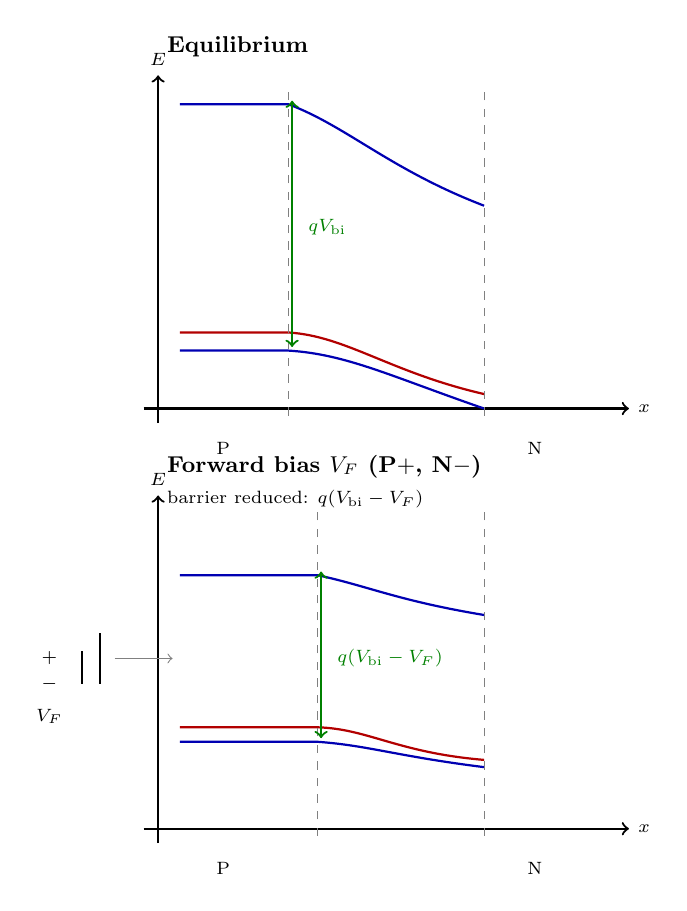
\begin{tikzpicture}[font=\small, scale=0.92, transform shape]

  % --- equilibrium ---
  \begin{scope}
    \node[anchor=west, font=\small\bfseries] at (0,5.0) {Equilibrium};
    \draw[->, thick] (-0.2,0) -- (6.5,0) node[right, font=\scriptsize] {$x$};
    \draw[->, thick] (0,-0.2) -- (0,4.6) node[above, font=\scriptsize] {$E$};

    \draw[thick, blue!70!black] (0.3,4.2) -- (1.8,4.2)
      .. controls (2.6,3.9) and (3.2,3.3) .. (4.5,2.8);
    \draw[thick, blue!70!black] (0.3,0.8) -- (1.8,0.8)
      .. controls (2.6,0.75) and (3.2,0.45) .. (4.5,0.0);
    \draw[red!70!black, thick] (0.3,1.05) -- (1.8,1.05)
      .. controls (2.6,1.0) and (3.2,0.5) .. (4.5,0.2);

    \draw[dashed, gray] (1.8,-0.1) -- (1.8,4.4);
    \draw[dashed, gray] (4.5,-0.1) -- (4.5,4.4);
    \draw[<->, green!50!black, thick] (1.85,4.25) -- (1.85,0.85);
    \node[font=\scriptsize, green!50!black, anchor=west] at (1.95,2.5)
      {$qV_{\mathrm{bi}}$};
    \node[font=\scriptsize] at (0.9,-0.55) {P};
    \node[font=\scriptsize] at (5.2,-0.55) {N};
  \end{scope}

  % --- forward bias ---
  \begin{scope}[yshift=-5.8cm]
    \node[anchor=west, font=\small\bfseries] at (0,5.0)
      {Forward bias $V_F$ (P$+$, N$-$)};
    \node[font=\scriptsize, anchor=west] at (0,4.55)
      {barrier reduced: $q(V_{\mathrm{bi}}-V_F)$};

    \draw[->, thick] (-0.2,0) -- (6.5,0) node[right, font=\scriptsize] {$x$};
    \draw[->, thick] (0,-0.2) -- (0,4.6) node[above, font=\scriptsize] {$E$};

    % less bending
    \draw[thick, blue!70!black] (0.3,3.5) -- (2.2,3.5)
      .. controls (2.9,3.35) and (3.3,3.15) .. (4.5,2.95);
    \draw[thick, blue!70!black] (0.3,1.2) -- (2.2,1.2)
      .. controls (2.9,1.15) and (3.3,1.0) .. (4.5,0.85);
    \draw[red!70!black, thick] (0.3,1.4) -- (2.2,1.4)
      .. controls (2.9,1.38) and (3.3,1.05) .. (4.5,0.95);

    \draw[dashed, gray] (2.2,-0.1) -- (2.2,4.4);
    \draw[dashed, gray] (4.5,-0.1) -- (4.5,4.4);

    \draw[<->, green!50!black, thick] (2.25,3.55) -- (2.25,1.25);
    \node[font=\scriptsize, green!50!black, anchor=west] at (2.35,2.35)
      {$q(V_{\mathrm{bi}}-V_F)$};

    % battery symbol
    \draw[thick] (-0.8,2.0) -- (-0.8,2.7);
    \draw[thick] (-1.05,2.0) -- (-1.05,2.45);
    \node[font=\scriptsize] at (-1.5,2.35) {$+$};
    \node[font=\scriptsize] at (-1.5,2.0) {$-$};
    \node[font=\scriptsize] at (-1.5,1.55) {$V_F$};
    \draw[->, gray] (-0.6,2.35) -- (0.2,2.35);

    \node[font=\scriptsize] at (0.9,-0.55) {P};
    \node[font=\scriptsize] at (5.2,-0.55) {N};
  \end{scope}

\end{tikzpicture}
\end{document}
